\documentclass[sigconf,authorversion,nonacm, 11pt]{acmart}

\usepackage{blindtext}
\usepackage{multicol}
\usepackage{array}
\usepackage{caption}
\usepackage{wrapfig}
\usepackage{listings}
\usepackage{caption}
\usepackage{subcaption}
\usepackage{acronym}
\usepackage{amsmath}
\usepackage{cleveref}
\usepackage{mathtools}
\usepackage{makecell}
\usepackage{booktabs} 
\usepackage{balance}
\usepackage{xspace}
\usepackage{balance}
\usepackage{circledsteps}
\usepackage{textcomp}
\usepackage{amsmath,amssymb,amsfonts}
\usepackage{graphicx}
\usepackage{textcomp}
\usepackage{xcolor}
\usepackage{multirow}
\usepackage{algpseudocode}
\usepackage{algorithm}

\acrodef{fsm}[FSM]{Finite State Machine}
\acrodef{dsa}[DSA]{Domain-Specific Architecture}
\acrodef{rei}[REI]{Regular Expression Inference}
\acrodef{ml}[ML]{Machine Learning}
\acrodef{ssa}[SSA]{Static Single-Assignment}
\acrodef{re}[RE]{Regular Expression}
\acrodef{nlp}[NLP]{Natural Language Processing}
\acrodef{ast}[AST]{Abstract Syntax Tree}
\acrodef{fsa}[FSA]{Finite State Automaton}
\acrodef{itp}[ITP]{Interactive Theorem Proving}
\acrodef{cegar}[CEGAR]{Counterexample-Guided Abstraction Refinement}


\acrodef{gpu}[GPU]{Graphic Processing Unit}
\acrodef{fpga}[FPGA]{Field Programmable Gate Array}
\acrodef{rtl}[RTL]{Register Transfer Level}
\acrodef{ir}[IR]{Intermediate Representation}

\begin{document}

\title{Democratizing Hardware Verification By Formalizing High-Level Abstractions}

\author{Luisa Cicolini}

\maketitle
\thispagestyle{empty}

\textit{
    Hardware verification is a fundamental step of the hardware design process, preventing expensive and potentially critical 
    mistakes.
    As the complexity of hardware designs increases, so does the need for more efficient verification strategies that can 
    make the overall design procedure smoother. % smoothen the overall...?
    In this context, exploiting higher-level hardware representations can be a game changer in verifying the designs 
    progressively during their lowering and explore different verification approaches that do not work with 
    lower-level hardware representations. % the part after the and doesnt make sense gramamtically, rephrase.
    However, efficiently extracting such high-level information remains a challenge due to the lack of formalized semantics  
    for high-level abstractions, which often rely on very specific structures, for example, \acp{fsm}.
    With this work, I aim to build the necessary infrastructure that can exploit such information,
    by formalizing the semantics of different hardware abstractions within the CIRCT ecosystem, to 
    (1) extract relevant higher-level information that can guide lower-level verification efforts, 
    (2) verify (parts of) the CIRCT compiler itself, % and?
    (3) explore different approaches to the verification of higher-level representations, thus distributing verification 
    efforts throughout the overall design procedure. 
}


\section{Introduction}

\begin{figure*}[ht]
    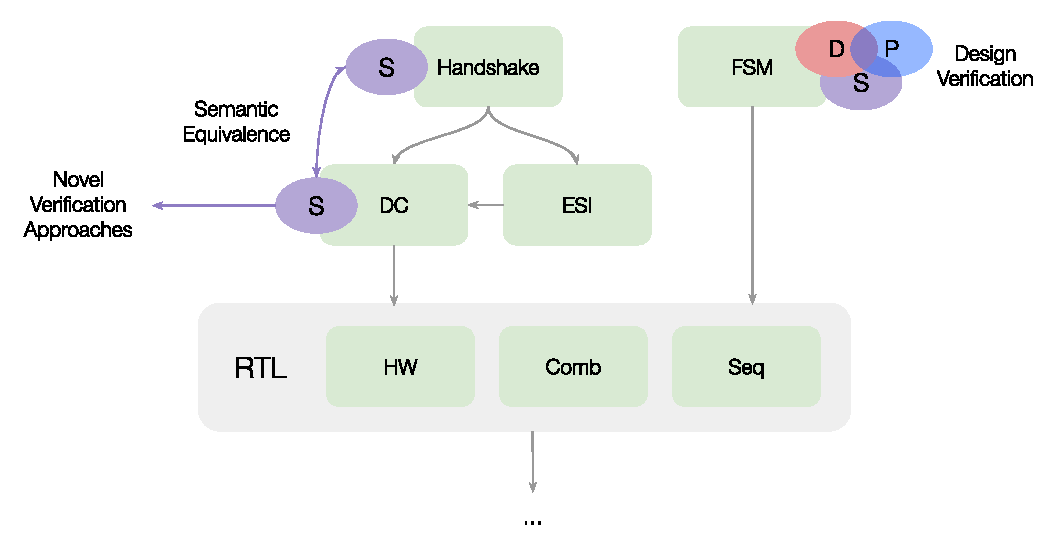
\includegraphics[scale=0.8]{semantics.pdf}
    \caption{Formalizing the semantics (S) of CIRCT dialects in Lean4 allows us to (1) verify the compilation and equivalence 
    between different abstractions, (2) explore novel verification approaches in a verified environment, (3) verify whether a property  % verification approaches in verified environment sounds weird
    (P) holds for a design (D) at a certain level.}
\end{figure*}

Hardware design is inherently complex, requiring a thorough understanding of numerous components and tools. 
Verification is crucial in the design process as it can uncover expensive and potentially critical mistakes before the tape-out.
The CIRCT project~\cite{circt, mlir_circt} introduces a novel concept of hardware compiler, comprising different domain-specific abstractions (\textit{dialects}),  %concept->conception maybe
frontends and backends that make the compilation of a design progressive, through numerous lowerings among different dialects.  % among -> through?
Exploiting these abstractions allows the designers to reason about different aspects of the design separately and introduce various 
optimizations at different levels of abstraction.
In brief, CIRCT~\cite{circt, mlir_circt} allows the progressive compilation of high-level abstractions, such as Finite State Machines, into lower-level representations, 
such as Verilog, via different lowerings. 
This approach proved successful in increasing the reusability of the code and introducing specific optimizations at different abstraction levels, 
by relying on the progressive lowering of the code. 
Being able to optimize and reason about a design at various abstraction levels is especially appealing from a hardware 
designer's perspective. 
Moreover, CIRCT's higher-level abstractions provide valuable information about the design's structure, 
which is available to perform preliminary verification tasks at a higher level, verify the compilation itself, 
and extract useful information that can serve lower-level verification tools~\cite{huang2018instruction, chen2021leveraging, mattarei2018cosa}. 

\textbf{Taking advantage of high-level abstractions is fundamental to building a verification toolchain that fully exploits the unique characteristics 
of the CIRCT ecosystem}, allowing designers to leverage the expressive power of different representations, for example, dataflow and \ac{fsm}. 
However, extracting useful high-level information remains a complex task due to the scarce formalization and the lack of precise 
semantics for CIRCT dialects. Overall, accurately formalizing the semantics of such diverse dialects and abstractions remains a 
significant challenge and is critical for verifying the correctness of the designs, optimizations and lowerings involved in the compilation. 



\section{Related Work}

Given the paramount importance of verification in hardware design, numerous works tackled the formalization and definition of 
semantics in hardware description languages, considering different levels of abstraction~\cite{melham1988abstraction}. 
Koika~\cite{bourgeat2020essence} directly derives from Bluespec~\cite{bluespec} and features novel and deterministic operational semantics, 
including a verified compiler to circuits. In particular, Koika highlights the importance of cycle-accurate description (and semantics) 
when dealing with the performance of circuits without compromising on the straightforward description of their functional properties. 
In particular, the authors highlight how traditional HDLs and HLS compilers lack precise semantics, making it especially hard to 
describe complex interactions between different modules.
ReWire~\cite{procter2015semantics} introduces a functional programming language with a compiler that translates the high-level 
description of a design into working hardware relying on the language's semantics to describe its behaviour.
Chisel~\cite{bachrach2012chisel} is another powerful structural language embedded in Scala, also used as a frontend for CIRCT. 
Finally, Bernstein et al. ~\cite{bernstein2021semantics} suggest exploiting abstract interpretation to formalize and represent 
different hardware abstractions, which require focusing on different aspects of the semantics. 
% In particular, this work considers the differences in event-based semantics (e.g. the ones commonly used for dataflow abstractions) 
% and semantics derived from sequential code description languages (e.g. in HLS workflow). 
The authors use abstract interpretation to describe the semantics at different levels of abstraction, 
mainly focusing on the representations used in the early phase of the design when reasoning at the latency-insensitive level of the hardware representation.
In particular, the semantics of latency-insensitive abstractions and their relationship to cycle-based representation are incredibly challenging. 
In this context, Carloni et al. ~\cite{carloni2001theory} introduce a theory to describe and represent latency-insensitive circuits and systems. 
The idea is to represent complex systems considering their single functional components and communication according to a specific protocol. 
The theory introduced allows for the composition of such single components into a complex system to satisfy synchronization and communication properties. 

Overall, these works focus on precise abstraction levels - either low or high. 
Instead, the CIRCT compilation toolchain exposes different abstraction at different levels: 
reasoning about their semantics allows \textbf{taking advantage of CIRCT’s flexible approach to hardware design}, complementing it with solid correctness 
guarantees concerning the designs and, ultimately, the compilation itself.

Due to the complexity of its environment, correctness guarantees in CIRCT require careful reflection on the semantics of the various \acp{ir} involved and the lowerings between them. 
To tackle this problem, CIRCT features different lowerings to standard hardware verification formats, such as \texttt{btor2}~\cite{btor2, niemetz2018btor2}, \texttt{aig}~\cite{aiger2} and \texttt{SMT-LIB}~\cite{barrett2010smt}, 
that contribute to integrating verification within the hardware design process.
In particular, the SMT dialect represents one means towards formalizing dialects' semantics at different levels. 
In fact, this dialect comprises most SMT-LIB~\cite{barrett2010smt} operators and is the endpoint of various lowerings from different dialects, 
meaning that their semantics is encoded in SMT-LIB and can be exported to SMT-LIB for verification.
The dialect is part of the compiler verification and optimization efforts currently under development in a research group at the 
University of Cambridge, with whom I have worked for the past year. 
However, the underlying complexity of SMT makes it hard to embed such domain-specific information into the actual SMT model~\cite{gurfinkel2022program}.
\texttt{circt-lec} and \texttt{circt-bmc} are other tools that perform logical equivalence checking and bounded model checking, respectively, at the \ac{rtl} level. 
Another recent work~\cite{zhao2024k} provided a preliminary formalization of CIRCT dialects, only focusing on lower-level \acp{ir}. 
While the current CIRCT infrastructure features various efforts toward the verification of the toolchain and its design, none of these 
take full advantage of CIRCT's high-level abstractions and eventually always fall back to lower-level representations.  

Works such as Lean-MLIR~\cite{bhat2024verifying} have already proved the benefits 
of embedding dialects' semantics in Lean4, an open-source programming language and theorem prover providing a flexible environment to write verified code. 
In fact, when using typical verification methods, such as SMT and SAT solvers, we need to put a lot of trust in their correctness. 
As an example, consider z3~\cite{de2008z3}: it consists of a huge C++ codebase, it is not verified, and these characteristics make the extension
of its tactics and logics incredibly hard. 
As a consequence, optimizing the job of the SMT solver, for example by introducing tactics that exploit domain-specific knowledge available at 
higher abstraction levels is not a practically viable solution. 
Instead, Lean4 provides a flexible and verified environment to expand CIRCT's verification tooling, 
making it possible to write theorems that encode certain domain-specific behaviours and successfully guide the verification, 
with a significantly higher degree of trust. 
This characteristics also makes Lean4 the perfect environment to experiment with further, verified verification 
methods, for example abstract interpretation.
Lean4 already proved very effective in building white-box automation techniques for bitvectors manipulation (to which I contributed)
and verification. 
In particular the \texttt{bv\_decide} tactic~\cite{bvdecide} represents a first effort in this space, implementing a verified bitblaster and 
LRAT checker. 
This fact demonstrates the potential of Lean4 in the field of verification and the interest of the community in working towards this direction. 

\section{Research Direction and Challenges}

During my PhD, I aim to enhance verification efforts for the CIRCT infrastructure by formalizing the semantics of its dialects 
to enable the verification of lowerings and optimizations, the adoption of novel verification techniques, 
and the progressive verification of designs' properties. 
Following the direction indicated by Lean-MLIR~\cite{bhat2024verifying}, I intend to formalize more high-level abstractions and dialects, 
starting from the Finite State Machine (FSM) dialect, and also considering those relying on radically different design paradigms 
from traditional imperative or functional IRs, such as the Dynamic Control (DC) dialect. 
This aspect will require careful mathematical modelling of complex, dataflow-like behaviour to fill gaps in the informal model, e.g. where latency-insensitive and 
circuit-based semantics meet. 
Besides introducing a powerful means to reason about dialects' semantics and the overall correctness of the compilation, 
this work will also lay the foundations for including higher-level verification techniques into CIRCT, for example, those leveraging automata-theoretic 
and abstract-interpretation-based approaches. 

This work takes advantage of CIRCT's great potential, lying in the high-level information available at different abstraction levels it provides, 
and combines it with Lean4's flexibility and trust. 
Until now, encoding high-level information in standard lower-level hardware verification techniques 
(such as assertion-based verification or SMT solvers) has been very complex ~\cite{symbiyosys, witharana2022survey}, 
due to the scarce flexibility of the tools involved (e.g. z3~\cite{de2008z3}) and the limited number of abstractions they support. 
With this work, the high-level information we extract by accurately formalizing dialects' semantics can contribute to guiding the effort of lower-level, 
classical verification approaches.   
In fact, Lean4 makes it possible to write verified theorems that extract and exploit the domain-specific information 
available at higher abstraction levels. 
The formalization of dialects within Lean4 also enables the verification of compiler passes, offering further guarantees for the correctness
of CIRCT itself. 

Moreover, formalizing the semantics of CIRCT dialects allows semantics manipulation up to a point where the application of different verification approaches is possible and beneficial. 
Exploring different approaches in the context of hardware verification is currently a challenge~\cite{mukherjee2015hardware, malik2008hardware}, requiring significant effort to bridge the hardware level 
with a suitable abstraction that can be digested by alternative verification methodologies, such as abstract interpretation frameworks. 
Nevertheless, preliminary studies suggested the effectiveness of these methodologies, 
especially at specific abstraction levels~\cite{bernstein2021semantics}. 
Formalizing the semantics of CIRCT dialects is a game-changer in this context, the more so when the formalization 
lives in a verified environment such as the one Lean4 offers. 



Lean4 is a fertile and open-source environment to work on verification frameworks thanks to its flexibility, versatility and trust level. 
Moreover, working in an open-source environment is an incredibly valuable aspect of this work, as it significantly increases the quality of the output - thanks to peer-review processes - 
and creates impact, being available to numerous users.  

Overall, formalizing the semantics of a large subset of CIRCT's dialects is a first step towards integrating the EDA toolchain with automatic verification, 
which is simultaneous and progressive with the design procedure and comprises different verification techniques. 
While this aspect can increase the compilation time for a single design iteration, 
its correctness guarantees can significantly reduce the number of iterations required to generate the desired design, 
eventually improving the overall design pipeline.
This work paves the way for filling and reasoning about subtle semantics gaps in hardware abstractions, by introducing formally verified semantics 
in the CIRCT ecosystem.

\section{Research Organization}

This research proposal comprises three milestones, which I plan to distribute in the three years of the PhD: 
\begin{enumerate}
    \item The goal of the first year is to \textbf{formalize the semantics of a first subset of high-level CIRCT dialects} (namely FSM, Handshake and DC) 
 and \textbf{verify their lowering to RTL level within Lean-MLIR}. This step is fundamental for the verification of the entire compilation. 
 To achieve this goal, I will spend the first four months of the PhD implementing in Lean4 the semantics of two high-level dialects (FSM, DC) and 
 the optimizations they involve. This phase will require careful study of existing works, especially concerning the formalization of latency-insensitive 
 behaviours in DC and their interface with cycle-accurate representation. 
 Subsequently, I will spend the next three months implementing the semantics of the CIRCT dialects necessary for the RTL-level representation (Hardware, Comb, Seq). 
 One more month will be necessary to tackle the engineering aspects involved in combining all these dialects in the Lean-MLIR framework and ensuring they work 
 flexibly and their integration is functional. I will spend the last four months of the first year proving the correctness of the lowerings from the higher-level 
 abstractions to RTL, including the optimizations involved. 
    \item \textbf{Bringing designs’ verification at a higher abstraction level, exploiting different dialects and their formalized semantics}. 
 At this point, a crucial step is understanding how to correctly specify relevant properties, which will require thorough readings in the State of the Art. 
 Moreover, I plan to add further dialects to the Lean-MLIR framework during the second year. 
    \item \textbf{Explore different verification strategies}, such as automata-theoretic approaches and abstract interpretation frameworks, 
 to fully take advantage of the formalized semantics. During the last year, I plan to take advantage of the effort put into effectively formalizing CIRCT dialects. 
 I will investigate how other verification techniques can further take advantage of the formalized semantics to improve the 
 guarantees concerning the design’s behaviour, aiming to reduce the number of necessary iterations. 
 I will also devote part of the last year to writing the PhD thesis, which will focus on how CIRCT and Lean4 are 
 a unique combination of tools to make hardware verification flexible and extensible, bending its tools to fit 
 different designs and techniques.
\end{enumerate}

\thispagestyle{empty}
\bibliographystyle{acm}
\bibliography{biblio}
\thispagestyle{empty}
\end{document}
